


\begin{abstract}
% This report presents a multiplayer first-person gaming platform built on an IoT architecture, using PYNQ-Z1 FPGA development boards as client nodes and a cloud-authoritative EC2 reactor server with a four-stage pipeline, backed by a three-tier persistence layer. Each node's ARM Cortex-A9 reads button inputs, computes player position and camera angle, and synchronises state with the server over UDP. The server acts as ground truth for all game state, broadcasting remote player and landmark coordinates back to each node, and doubles as a game development environment providing map creation and session management features. Received state is written into shared BRAM alongside local player data, where the Zynq-7000 programmable logic executes a DDA-based raycasting engine entirely in synthesised hardware, rendering the full scene in real time. The result is PYNQcast: both a fully playable multiplayer game and an operator-facing development environment, demonstrating hardware-accelerated rendering, bidirectional multi-node communication, and cloud-authoritative state management within an IoT framework.

PYNQcast is a multiplayer first-person raycasting game engine and 
cloud-hosted development platform built on an IoT architecture. 
PYNQ-Z1 FPGA nodes render scenes entirely in synthesised hardware, 
synchronising with a cloud-authoritative EC2 server over UDP. The 
server resolves game state across all nodes and exposes a 
browser-based development environment; demonstrating hardware-accelerated rendering, 
bidirectional multi-node communication, and cloud-authoritative state 
management within an IoT framework.


% \begin{figure}[H]
%     \centering
%     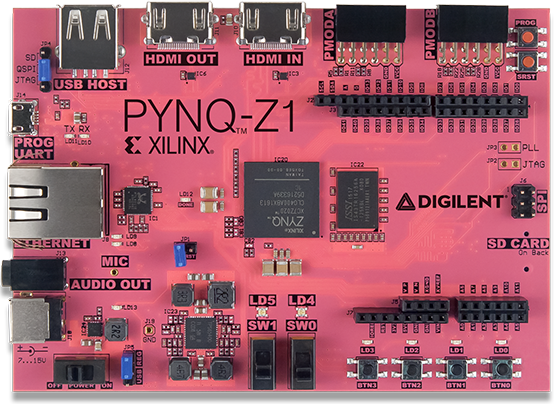
\includegraphics[width=0.5\linewidth]{images/pynq-z1-1.png}
%     \caption{PYNQ-Z1 dev board: Xilinx Zynq-7000 SoC; PS (dual-core ARM Cortex-A9) and PL (FPGA fabric).}
%     \label{fig:pynq_board}
% \end{figure}
\end{abstract}


